\documentclass[../uilmath.tex]{subfiles}
\graphicspath{{\subfix{../figures/}}}
\begin{document}
\chapter{Geometry}
\section*{Problems}
\begin{enumerate}[label=\bfseries\arabic*.]
    \item %% Problem 1
    The sides of a triangle are 9 in, 12 in, and 15 in. The triangle is a(n) \blank triangle:

    \item %% Problem 2
    An isosceles trapezoid has a top base of 8 cm, a bottom base of 14 cm, and a slanted side length of 5 cm. Find the area of the isosceles trapezoid.

    \item %% Problem 3
    Rene drew $\triangle ABC$ using the coordinates $(1,2), (2,-2)$ and $(5,1)$. Find the area of Rene's triangle.

    \item %% Problem 4
    Georg Alexander picks the special figure and places it on a five-peg-by-five-peg geoboard. Find the area enclosed by the figure.
    \begin{center}
        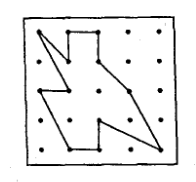
\includegraphics[width=0.3\textwidth]{2006SAC16.PNG}
    \end{center}

    \item %% Problem 5
    $\triangle DEF$ is an obtuse isosceles triangle such that m$\angle DEF$ is 104$\degree$ and EF is 14 cm. Find the area of $\triangle{DEF}$ to the nearest integer.

    \item %% Problem 6
    Point $P(3,3)$ is rotated 270$\degree$ counterclockwise about the origin to point $Q$. Point $Q$ is reflected across the $y$-axis to point $R$. Find the coordinates of point $R$.

    \item %% Problem 7
    Two chords, $AC$ and $BD$ intersect in the interior of a circle at point $X$ such that $m\arc{BC}=20\degree$ and $m\arc{AD}=120\degree$. If points $B$ and $C$ are not on $\arc{AD}$ then $m\angle AXD$ is:

    \item %% Problem 8
    The adjacent dots on the grid are 1 cm apart when measured vertically and horizontally. Find the area of the shaded figure shown.
    \begin{center}
        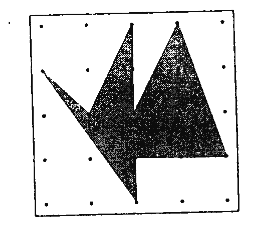
\includegraphics[width=0.3\textwidth]{2008SAC9.PNG}
    \end{center}

    \item %% Problem 9
    One of the base angles of an acute isosceles triangle has a measure of 50$\degree$ and the length of its base is 6 cm. Find the perimeter of the acute isosceles triangle. (nearest tenth)

    \item %% Problem 10
    The square below is divided into 5 congruent rectangles. The perimeter of each of the congruent rectangles is 30 units. What is the perimeter of the square?
    \begin{center}
        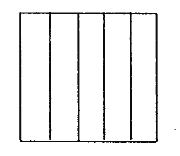
\includegraphics[width=0.3\textwidth]{2008SAC23.PNG}
    \end{center}

    \item %% Problem 11
    Simplify: $\frac{n!+(n-1)!}{(n-2)!}$

    \item %% Problem 12 
    Let $AB$ be the diameter of the circle with center $C$ with $CG\perp AB, DE\perp AB$, and $EF\perp DC$. 
    If $AE=9$ and $BE=4$ then $DE=$?
    \begin{center}
        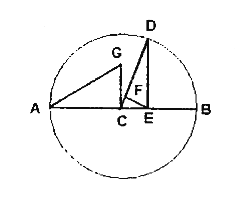
\includegraphics[width=0.3\textwidth]{2008SAC27.PNG}
    \end{center}

    \item %% Problem 13
    Given: $\triangle ABC \sim \triangle DEF, AB = 15, AC = 12, m\angle A = 62\degree, DE = 10$. $EF=\blank$. (nearest tenth)

    \item %% Problem 14
    Points $A$ and $B$ line on a circle with center $O$. The area of the circle is 531 and $AB=24$. Find the distance from $O$ to chord $\overline{AB}$. (nearest tenth)

    \item %% Problem 15
    Consider a circle circumscribed about a regular pentagon. If the area of the circle is 452.4, then the area of the pentagon is $\blank$. (nearest whole number)


    Use the sketch below for problems 16 and 17. The information given in problem 16 does not carry over to problem 17.
    \begin{center}
        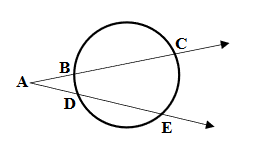
\includegraphics[width=0.3\textwidth]{2021SAC18.PNG}
    \end{center}
    \item %% Problem 16
    If $AB=6, BC=15$, and $AD=8$, then $DE=\blank$. (nearest hundredth)

    \item %% Problem 17
    If $mBD = 28\degree$ and $mCE = 86\degree$, then $m\angle CAE=\blank$.$\degree$

    \item %% Problem 18
    The base of a pyramid is a square with each side equal to three-fifths of the height of the pyramid. If the volume 
    of the pyramid is 700, what is the total area of the pyramid? (nearest whole number)

    \item %% Problem 19
    Angles $A$ and $B$ are complementary angles while angles $A$ and $C$ are supplementary angles. If 
    $m\angle A = 6x+1$ and $m\angle B = 9x-1$, then $m\angle C = \blank\degree$.

    \item %% Problem 20
    Quadrilateral $ABCD$ shown below is a square. The midpoint of $\overline{AD}$ is point $E$ and the midpoint of 
    $\overline{AB}$ is point $F$. If $EF=18$, then the area of the square is \blank.

    \begin{center}
        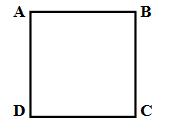
\includegraphics[width=0.3\textwidth]{2021SAC28.PNG}
    \end{center}

    \item %% Problem 21
    Consider a quadrilateral with vertices $A(-6,4), B(0,-8), C(6,4)$, and $D(0,12)$. This quadrilateral can be classified as a \blank.

    \item %% Problem 22
    Consider $\triangle ABC$ with point $D$ on $\overline{AB}$ such that $\overline{CD}\perp \overline{AB}$. If $m\angle ACB=78.28\degree$, $AD=9$ and $CD=12$, then $DB=\blank$. (nearest tenth)
    
    \item %% Problem 23
    Find the area of a triangle with vertices $(0,12), (0,0)$ and $(12,0)$.

    \item %% Problem 24
    If you cut nine circles out of a square piece of cardboard that measures 12 in by 12 in, how much cardboard is discarded? (nearest tenth)
    \begin{center}
        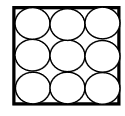
\includegraphics[width=0.3\textwidth]{2021SAC56.PNG}
    \end{center}

    \item %% Problem 25
    Russell's backyard pool is shaped like a rectangle that measures 30 ft by 50 ft. He decides to add a sidewalk that is 3 feet wide around the perimeter. Vedant, Caleb
    and Curtis will provide free labor, so he only has to pay for the concrete, which cost \$6.00 per square foot. What will the sidewalk cost?
    \begin{center}
        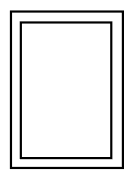
\includegraphics[width=0.3\textwidth]{2021SAC58.PNG}
    \end{center}

    \item %% Problem 26
    Find the area of the polygon below. (nearest whole number)
    \begin{center}
        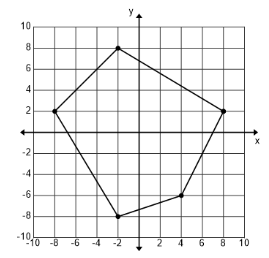
\includegraphics[width=0.3\textwidth]{2021SAC59.PNG}
    \end{center}


    The following polygon is used for problem 27 and 28.
    \begin{center}
        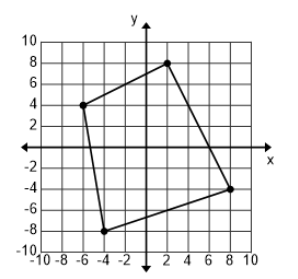
\includegraphics[width=0.3\textwidth]{2022SAC11.PNG}
    \end{center}
    \item %% Problem 27
    Find the perimeter of the polygon shown. (nearest tenth)

    \item %% Problem 28
    Find the area of the polygon shown.

    \item %% Problem 29
    Consider $\triangle ABC$ with $AB=18$ and $BC=14$. Point $D$ lies on $\overline{AC}$ such that $\overline{BD}$ bisects $\angle ABC$. 
    If $AD=10$, then $DC=\blank$. (nearest tenth)


    Use the following sketch for problems 30 and 31.
    \begin{center}
        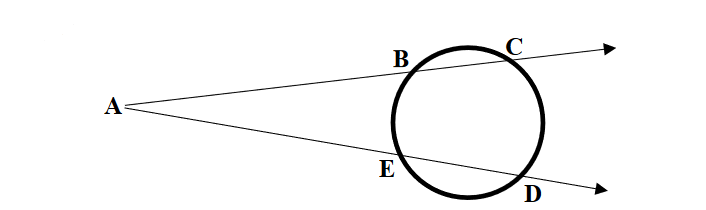
\includegraphics[width=0.3\textwidth]{2022SAC14.PNG}
    \end{center}
    \item %% Problem 30
    If $m\angle CAD=19\degree$, $mCD=120\degree$, $mDE=102\degree$, then $mBC=\blank$.

    \item %% Problem 31
    If $\overline{BD}$ intersects $\overline{CE}$ at point $P$ (not shown) with $BP=x+1$, $CP=2x$, $DP=2x+2$, and $EP=x+4$, then $CE=\blank$. (nearest tenth)

    \item %% Problem 32
    Consider a right circular cone with a base perimeter of 75 cm and a lateral area of 490 cm. Find the volume of the cone. (nearest whole number)

    \item %% Problem 33
    Consider a circle inscribed in a square with side lengths 44.6 mm. Find the area inside the square but outside the circle. (nearest whole number)

    \item %% Problem 34
    Find the perimeter of a regular decagon that can be inscribed in a circle with an area of 254 cm$^2$. (nearest tenth)

    \item %% Problem 35
    
    
\end{enumerate}

\section*{Solutions}
\begin{enumerate}[label=\bfseries\arabic*.]
    \item %% Problem 1
    Right 

    \item %% Problem 2
    44 cm$^2$

    \item %% Problem 3
    7.5 units$^2$

    \item %% Problem 4
    8 units$^2$

    \item %% Problem 5
    95 cm$^2$

    \item %% Problem 6
    $(-3,-3)$

    \item %% Problem 7
    70$\degree$

    \item %% Problem 8
    6 cm$^2$

    \item %% Problem 9
    15.3 cm 

    \item %% Problem 10
    50 units 

    \item %% Problem 11
    $n^2-1$

    \item %% Problem 12
    6

    \item %% Problem 13
    9.4

    \item %% Problem 14
    5.0

    \item %% Problem 15
    342

    \item %% Problem 16
    7.75 

    \item %% Problem 17
    29$\degree$

    \item %% Problem 18
    523

    \item %% Problem 19
    143

    \item %% Problem 20
    648

    \item %% Problem 21
    kite 

    \item %% Problem 22
    10.6

    \item %% Problem 23
    72

    \item %% Problem 24
    30.9 in$^2$

    \item %% Problem 25
    \$3096.00

    \item %% Problem 26
    148

    \item %% Problem 27
    47.2

    \item %% Problem 28
    136

    \item %% Problem 29
    7.8

    \item %% Problem 30
    56$\degree$

    \item %% Problem 31
    5.5

    \item %% Problem 32
    793 cm$^3$

    \item %% Problem 33
    427 mm$^2$

    \item %% Problem 34
    55.6 cm
    
    \item %% Problem 35
    
\end{enumerate}



\end{document}